\documentclass{article}
\usepackage[utf8]{inputenc}
\usepackage{url}
\usepackage{amsmath}
\usepackage{amssymb}
\usepackage{booktabs}
\usepackage{epsfig}
\usepackage{float}
\usepackage{hyperref}
\usepackage[inline]{enumitem}
\usepackage{graphicx}
\usepackage{listings}
\usepackage{multirow}
\usepackage[authoryear]{natbib}
\usepackage[margin=1in]{geometry}
\usepackage{amsthm}

\newtheorem{definition}{Definition}
\newtheorem{theorem}{Theorem}
\newcommand{\Fig}[1]{Fig.~\ref{fig:#1}\xspace}

\title{Strong Fairness}
% \author{}
% \date{25 March, 2022}
\date{\vspace{-5ex}}

\begin{document}

\maketitle
% \subsection{Strong Fairness}
% \label{ss:strong_fairness}
%\pg{Eashan verify if the theorems and are corollaries are indeed correct. Pay special attention to whether it should be $<$ ot $\leq$.}

\begin{definition}
An ordering process $O$ is strongly fair if it satisfies the following conditions,
\begin{align*}
    C1: &\text{ If } A_i(k) < A_i(l), \text{ then, } O(i,k) < O(i,l).\nonumber\\
    C2: &\text{ If } f_i(k) = f_j(l) \land rt_i(k) < rt_j(l), \text{ then, }
    O(i,k) < O(j,l).
\end{align*}
\label{def:strong}
\vspace{-5mm}
\end{definition}

%Condition $C1$ states that a MP is always better-off submitting the trade order as early as possible and waiting to submit trade orders does not offer any advantage.
Condition $C1$ states that a MP is always better-off submitting the trade order as early as possible. $C2$ states that trade orders generated based on the same market data point should be ordered based on the response time of the MPs.% (i.e., faster MP's trades should be ordered ahead).}
%$C2$ states that trade orders generated based on the same market data point should be ordered based on the response time of the MPs.} %.%forwarded to the ME first). 

\begin{theorem}
    The \textit{necessary} and \textit{sufficient} conditions on the delivery processes for strongly fair ordering are given by,
    \begin{align*}
        D_i(x+1) - D_i(x) &= D_j(x+1) - D_j(x), & \forall i,j,x.
    \end{align*}
    \label{thm:1}
    \vspace{-6mm}
\end{theorem}

The theorem states that for strong fairness the inter-delivery times should be the same across all  MPs. In other words, the delivery clocks at all RBs (at any given delivery clock time) must advance at the same rate.

% eg{The theorem states that, for strong fairness, the intervals between consecutive market data deliveries -- inter-delivery times -- should be the same across all MPs. In other words, the delivery clocks at all RBs (at any given delivery clock time) must advance at the same rate.}

\begin{proof}
\textit{Necessary:} To prove that the above condition is necessary we will show that if this condition is not met then no ordering process exists which is strongly fair for arbitrary trade orders. %\attn{We will constuct a tra}%already said this %
%The reason for this is that the OB does not know the response time of trade orders ($\sum f_i$ is unknown). 

\begin{figure}[b]
\centering
    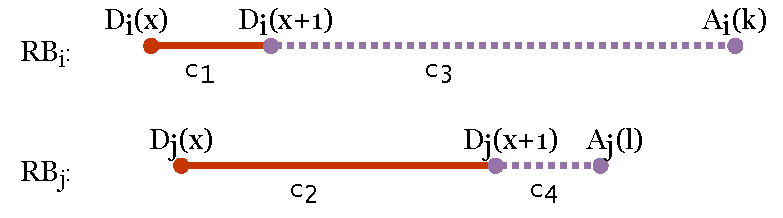
\includegraphics[trim={0 0 0 1mm},clip,width=0.9\columnwidth]{images/delivery times.pdf}
    \vspace{-3mm}
    \caption{{\small{\bf Proof of Theorem 1.}}}% \pg{Eashan include as an arrow for progress of time.}}
    \label{fig:proof}
    \vspace{-5mm}
\end{figure}

Consider the following scenario (\Fig{proof}) where the above condition is not met. Let $D_i(x+1) - D_i(x) = c1$, $D_j(x+1) - D_j(x) = c2$. Without loss of generality we assume $c1<c2$. Consider hypothetical trades $(i,k)$ and $(j,l)$ s.t. $A_i(k) = D_i(x+1) + c3$ and $A_j(l) = D_j(x+1) + c4$. Further, we can pick $A_i(k)$ and $A_j(l)$ s.t. $c3>c4$ and $c1+c3<c2+c4$. Now we consider two scenarios for how these trades were generated. These two scenarios are indistinguishable at the OB.
%Consider a hypothetical trade order $k$ (from MP$_i$) and $l$ (from MP$_j$) s.t. $A_i(k) = D_i(x+1) + c3$ and $A_j(l) = D_j(x+1) + c4$. Further, we can pick $A_i(k)$ and $A_j(l)$ s.t. $c3>c4$ and $c1+c3<c2+c4$. Now we consider two scenarios for how these trades were generated. These two scenarios are indistinguishable at the OB.

\noindent
\text{Case 1:} $f_i(k) = f_j(l) = x+1$. Here,
\begin{align}
rt_i(k) = c3, rt_j(l) = c4.
\end{align}
Since $c3>c4$, a strongly fair ordering (condition $C2$) must satisfy,
%\begin{align}
$O(i,k) > O(j,l)$.
%\label{eq:theorem_1:necessary:case1}
%\end{align}

\noindent
\text{Case 2:} $f_i(k) = f_j(l) = x$. Here,
\begin{align}
rt_i(k) = c1+c3, rt_j(l) = c2+c4.
\end{align}
In this case, since $c1+c3<c2+c4$, a strongly fair ordering must instead satisfy the opposite, $O(i,k) < O(j,l)$. A contradiction! \attn{Thus, no ordering process can be strongly fair in both these scenarios.}
%\label{eq:theorem_2:necessary:case1}
%\end{align}


\smallskip
\noindent
\textit{Sufficient:} We will now show that if the inter-delivery times are same across MPs, then a strongly fair ordering exists. 

Assuming same inter-delivery times, DBO trivially satisfies $C1$. DBO also satisfies $C2$, i.e.,  if $f_i(k) = f_j(l) \land rt_i(k) < rt_j(l)$, then,
\begin{align}
    DC_i(A_i(k)) < DC_j(A_j(l)). 
\end{align}
Intuitively, this is because market data $f_i(k) (= f_j(l))$ is delivered to each MP at the same delivery clock time (by definition). Further, delivery clocks advance at the same rate across all MPs. When measured from the delivery of $f_i(k) (= f_j(l))$, delivery clock of RB$_j$ in duration $rt_j(l)$ will advance more than delivery clock of RB$_i$ in duration $rt_i(k)$.
Therefore, DBO is strongly fair.\footnote{\attn{Note that, DBO is not the only ordering process that can achieve strong fairness. Other ordering processes that also order trades from MPs based on when they received the market data can also achieve strong fairness.}} 
\end{proof}

\if 0
Assuming same inter-delivery times, DBO trivially satisfies $C1$. DBO also satisfies $C2$. If $f_i(k) = f_j(l) \land rt_i(k) < rt_j(l)$, then,
\begin{align}
    DC_i(A_i(k)) < DC_j(A_j(l)). 
\end{align}
% \eg{
% \begin{align}
%     DC_i(A_i(k)) = \langle x^i_l, rt_i(k)+(D_i(f_i(k))-D_i(x^i_l)) \rangle < DC_j(A_j(l)) = \langle x^j_l, rt_j(l)+(D_j(f_j(l))-D_j(x^j_l)) \rangle. 
% \end{align}}
Intuitively, DBO satisfies $C2$ because market data $f_i(k) (= f_j(l))$ is delivered to all the MPs at the same delivery clock time (by definition). Because delivery clocks advance at the same rate across all MPs, (measured from the delivery of $f_i(k)$) delivery clock of RB$_j$ in duration $rt_j(l)$ will have advanced more than delivery clock of RB$_i$ in duration $rt_i(k)$.
Therefore, DBO is strongly fair. 
%\end{proof}
\fi

% \bibliographystyle{plain}
% \bibliography{egbib}
\end{document}

